\documentclass[tikz]{standalone}

\usepackage{amssymb}
\usetikzlibrary{shapes.geometric}

\begin{document}
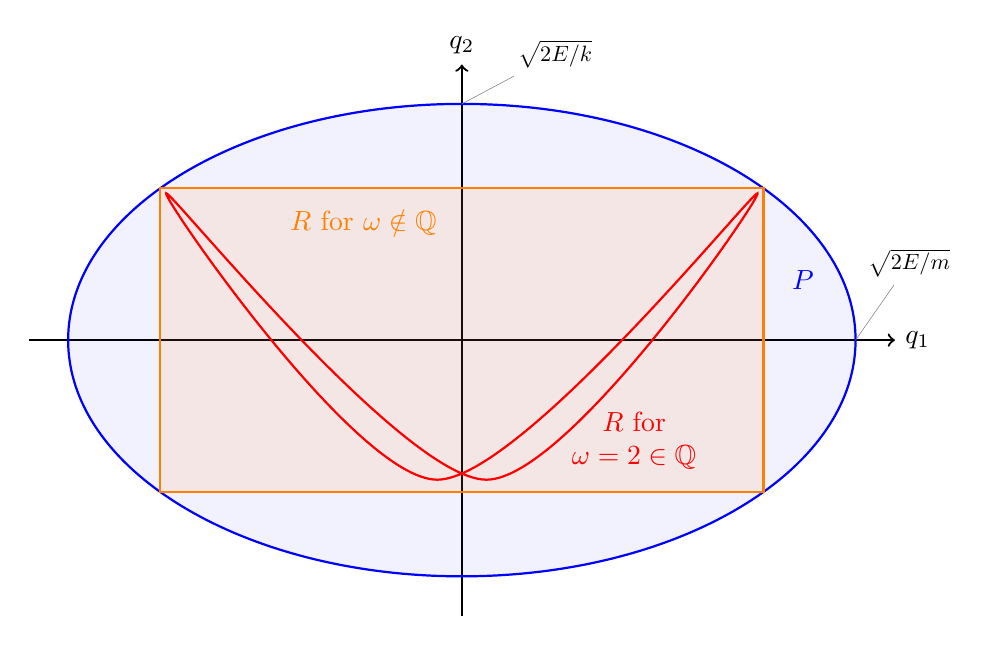
\begin{tikzpicture}[thick]

  % Axes
  \def\x{5}\def\y{3}
  \draw[->] (-\x-0.5,0) -- (\x+0.5,0) node[right] {$q_1$};
  \draw[->] (0,-\y-0.5) -- (0,\y+0.5) node[above] {$q_2$};

  % Ellipse
  \draw[blue,fill=blue,fill opacity=0.05] (0,0) circle [x radius=\x, y radius=\y];
  \coordinate[pin={[pin distance=25,scale=0.8]85:$\sqrt{2E/m}$}] (r1) at (\x,0);
  \coordinate[pin={[pin distance=25,scale=0.8]30:$\sqrt{2E/k}$}] (r2) at (0,\y);
  \node[blue] at (10:\x-0.6) {$P$};

  % Rectangle
  \draw[orange,fill=orange,fill opacity=0.1] (220:\x+0 and \y+0) rectangle (40:\x+0 and \y+0);
  \node[orange] at (-\x/4,\y/2) {$R$ for $\omega \notin \mathbb{Q}$};

  % Trajectory
  \draw[red] plot [smooth cycle] coordinates {(140:\x-0.1 and \y-0.1) (280:1.8) (40:\x-0.1 and \y-0.1) (260:1.8)} node[shift={(2.5,0.5)},align=center] {$R$ for \\$\omega = 2 \in \mathbb{Q}$};

\end{tikzpicture}
\end{document}